\documentclass{homework}
\usepackage{lipsum}
\usepackage{alltt}
\usepackage{cancel}
\usepackage{amsthm}
\usepackage{cleveref}
\usepackage{upgreek}
\usepackage{mathrsfs}
\usepackage{tikz}
\usepackage{units}
\usepackage{caption}
\usepackage{listings}
\usepackage{color} %red, green, blue, yellow, cyan, magenta, black, white
\usetikzlibrary{positioning}
\usetikzlibrary{graphs}

\DeclareMathOperator{\cov}{cov}

\title{Kevin Joyce}
\course{Math 491 - Big Data Analytics - Homework 2}
\author{Kevin Joyce}
\docdate{March 4, 2015}
\begin{document} 
\newcommand{\figref}[1]{\figurename~\ref{#1}}
\renewcommand{\bar}{\overline}
\renewcommand{\hat}{\widehat}
\renewcommand{\SS}{\mathcal S}
\newcommand{\HH}{\mathscr H}
\newcommand{\mom}{\widetilde}
\newcommand{\mle}{\widehat \Uptheta}
\newcommand{\eps}{\varepsilon}
\newcommand{\todist}{\stackrel{D}\longrightarrow}
\newcommand{\toprob}{\stackrel{p}\longrightarrow}
\newcommand{\TTheta}{\overline{\underline \Theta} }
\newcommand{\del}{\partial}
\newcommand{\approxsim}{\overset{\cdotp}{\underset{\cdotp}{\sim}}}
\newcommand{\RSS}{\ensuremath{\mathrm{RSS}}}
\newcommand{\MSE}{\ensuremath{\mathrm{MSE}}}
\newcommand{\SE}{\ensuremath{\mathrm{SE}}}
\newcommand{\TSS}{\ensuremath{\mathrm{TSS}}}
\newcommand{\Var}{\ensuremath{\mathrm{Var}}}
\newcommand{\SSReg}{\ensuremath{\mathrm{SSReg}}}
\renewcommand{\a}[1]{{\color{red} \it #1}}

\problem{
  Consider the following series of measurements of the unknown value $x$:
  $$
    y_i = a_i x + \eps_i, \quad = 1,\dots,n,
  $$
  where $y_i$ are measurement results, $a_i$ are known coefficients, and $\eps_i$ represent random error of measurement and are independent identically distributed (i.i.d.) with zero mean and variance $\sigma^2$:
  $$
    E\eps_i = 0, \quad E\eps_i^2 = \sigma^2, \quad i=1,\dots,n
  $$
} 

\subproblem{What function of $y_1,\dots,y_n$ (and of $a_1,\dots,a_n$) would you use as a good estimate for $\hat x$ for $x$?}

\begin{quote}
%A straight-forward estimate for $x$ would be to average the reciprocally weighted measurements, i.e.
%$$
%\hat x = \frac 1n\sum_{i=1}^n\frac{y_i}{a_i}.
%$$
  Although not obvious, a good estimate for $x$ would be 
  $$
  \hat x = \frac{\sum a_iy_i}{\sum a_i^2}.
  $$
  We will show in the next part that this estimate minimizes the sum of the squared distances to the measured data.
\end{quote}


\subproblem{Is this estimate optimal in any sense?}

\begin{quote}
For any given estimate $x$, the sum of the squared differences between observations and estimates of the observations is given by
$$
  Q(x) = \sum_{i=1}^n(y_i - a_i x)^2,
$$
for which
\begin{align*}
  Q(x) 
  &= \left(\sum a_i^2\right) x^2 - \left(2\sum a_iy_i\right)x + \sum y_i^2\\
  &= \left(\sum a_i^2\right) x^2 - \left(2\sum a_iy_i\right)x + \frac{\left(\sum a_iy_i\right)^2}{\sum a_i^2} - \frac{\left(\sum a_iy_i\right)^2}{\sum a_i^2} + \sum y_i^2 \\
  &\stackrel{\dagger}= \left( \left(\sum a_i^2\right)^{1/2} x - \frac{\sum a_iy_i}{(\sum a_i)^{1/2}} \right)^2 - \frac{\left(\sum a_iy_i\right)^2}{\sum a_i^2} + \sum y_i^2.
\end{align*}
Since only the first term depends on $x$, and each term is positive, $Q(x)$ is minimized when the first squared term vanishes. This happens precisely when 
$$
  \hat x = \frac{\sum a_iy_i}{\sum a_i^2} =:\frac UV,
$$
where $U$ and $V$ are the respective sums.
\end{quote}
  
\vspace{-1em}
\subproblem{Is it a biased or an unbiased estimate?}

Observe
\begin{align*}
   \hat x - x
   &= \left(\sum a_i^2\right)^{-1} \sum a_i (a_i x + \eps_i)  - x \\
   &= \left(\sum a_i^2\right)^{-1} \left(\sum a_i^2\right) x - x + \left(\sum a_i^2\right)^{-1} \sum a_i\eps_i\\
   &\stackrel*=\left(\sum a_i^2\right)^{-1} \sum a_i\eps_i.
\end{align*}
\vspace{-1em}
Taking expectations on both sides and using $E\eps_i = 0$, we see that $\hat x$ is unbiased for $x$.

\newpage
\subproblem{What is its variance (expressed through $\sigma^2$)?}

\begin{quote}
Since $E\hat x = x$, the variance of $\hat x$ is given by 
\begin{align*}
  \Var(\hat x) = E(\hat x - x)^2 
  &\stackrel*=E\left(\left(\sum a_i^2\right)^{-1} \sum a_i\eps_i\right)^2\\
  &=E\left(\left(\sum a_i^2\right)^{-2} \sum_{i,j} a_ia_j\eps_j\eps_i\right)\\
  &=\left(\sum a_i^2\right)^{-2} \sum_{i,j} a_ia_j E\eps_i\eps_j\\
  &=\left(\sum a_i^2\right)^{-2} \sum_{i} a_i^2 \sigma^2\\
  &=\frac{\sigma^2}{V} . 
\end{align*}
\end{quote}

\subproblem{How would you estimate $\sigma^2$ if it is unknown?}

\begin{quote}
  Continuing from the last line of the derivation of $\hat x$, we have
  \begin{align*}
    Q(\hat x) 
    &\stackrel\dagger= 0 + \sum y_i^2 - \frac{U^2}{V} \\
    &= \sum (a_i x + \eps_i) ^2 - V\hat x^2 \\
    &= \sum (x^2a_i^2 +2xa_i\eps_i + \eps_i^2) - V\hat x^2 \\
    &= 2x\sum a_i\eps_i + \sum \eps_i^2 - V(\hat x^2 - x^2). \\
    \intertext{Taking expectations on both sides and using $\frac{\sigma^2}{V} = E(\hat x - x)^2 = E\hat x^2 - 2xE\hat x + x^2 = E\hat x^2 - x^2$,we obtain}
    EQ(\hat x) &= 0 + n\sigma^2 - V \frac{\sigma^2}{V}\\
   &= (n-1)\sigma^2.
  \end{align*}
  Hence, an unbiased estimate of $\sigma^2$ is given by
  $$
  \hat{\sigma^2} = \frac{Q(\hat x)}{n-1} = \frac 1{n-1} \left(W - \frac{U^2}{V}\right),
  $$
  where $W = \sum y_i^2$.
\end{quote}

\subproblem{What would you use as an estimate for $\Var(\hat x)$ if $\sigma^2$ is unknown?}

\begin{quote}
  Based on (d) and (e), an unbiased estimate for $\Var(\hat x)$ is
  $$
  \hat{\Var(\hat x)} = \frac{\hat{\sigma^2}}{V} = \frac{1}{n-1}\left(\frac WV - \hat x^2\right)
  $$
\end{quote}

\subproblem{Suppose that the variance $\sigma^2$ is known.  What ``canonical information'' would be sufficient to extract from the series of observations
$$
(y_1,a_1),\dots,(y_n,a_n),\quad i = 1,\dots,n
$$
in order to compute the estimate $\hat x$, and its variance $\Var(\hat x)$?
}

\begin{quote}
  From the previous derivations, we need only the quantities $U = \sum a_iy_i$ and $V = \sum a_i^2$ to compute
  $$
  \hat x = \frac UV,\quad\text{and}\quad \Var(\hat x) = \frac{\sigma^2}{V}.
  $$
\end{quote}

\subproblem{ Suppose that the variance $\sigma^2$ is NOT known.  What ``canonical information'' would be sufficient to extract from the series of observations in order to compute $\hat x$,$\hat{\sigma^2}$, and $\hat{\Var(\hat x)}$.}

\begin{quote}
  From the previous derivations, we need only the quantities $U = \sum a_iy_i,V = \sum a_i^2,W = \sum y_i^2,$ and $n$ to compute
  $$
  \hat x = \frac UV,\quad\text{and}\quad \hat{\Var(\hat x)} = \frac 1{n-1}\left(\frac{W}{V} - \hat x^2\right).
  $$
\end{quote}

\subproblem{ How should we update such ``information'' when a new observation $(y_{n+1},a_{n+1})$ arrives? }

\begin{quote}
  Since each element of the canonical information is expressed as a sum, we can easily update via the following schematic:

  \begin{tikzpicture} 
    \draw[-latex]{ (0,0) node[left]{$(U,V,W,n)$} -- (1,0) node[right]{$\oplus$} };
    \draw[-latex]{ (1.55,0) node[right]{} -- (3,0) node[right]{$(U+y_{n+1}a_{n+1}, V+a_{n+1}^2, W+y_{n+1}^2,n+1)$} }; 
    \draw[-latex]{ (0,-.7)  node[below left]{$(y_{n+1},a_{n+1})$} -- (1,-.1) node[below left]{}};
  \end{tikzpicture}
\end{quote}

\subproblem{ How should we ``combine'' (merge) two pieces of ``canonical information''?}

\begin{quote}
  Again, because the canonical information is expressed through sums, information is easily combined via the following schematic:

    \begin{tikzpicture}[node distance=1em and 2em,>=latex]
    \node (plus) [] {$\oplus$};
    \node (in1) [above left=of plus] {$(U,V,W,n)$};
    \node (in2) [below left=of plus] {$(U',V',W',n')$};
    \node (combined) [right=of plus] {$(U+U',V+V',W+W',n+n')$};

    \draw[->]
      (in1) edge (plus)
      (in2) edge (plus)
      (plus) edge (combined) 
    ;
  \end{tikzpicture}
\end{quote} 

\newpage
\problem{Write a program which illustrates simple linear regression (or a more general variant of linear regression) and implements accumulation of canonical information.}

\subproblem{For some fixed parameters $a$ and $b$ (or, in a more general case $a_1,\dots,a_m$) generate a sequence of ``observations'' $(x_i,y_i)$:
$$ y_i = f(x_i) = \eps_i $$
where 
$$ f(x) = a + bx\quad\text{or}\quad f(x) = a_1 + a_2x + a_3x^2 + \cdots + a_mx^{m-1} $$
$\eps_i$ are i.i.d. with zero mean and $\mathrm E \eps_i^2 = \sigma^2$. Values $x_i$ can be generated randomly with some mean and variance.
}

\subproblem{Accumulate canonical information, i.e., at each step when a new observation $(x_i,y_i)$ is produced update canonical information.}

\subproblem{Illustrate $\hat{f(x)}$.}

\subproblem{Illustrate $\Var(\hat{f(x)})$, assuming that $\sigma^2$ is known.}

\subproblem{Illustrate $\hat{\Var\hat{f(x)})}$, assuming that $\sigma^2$ is NOT known.}

In your repoprt present the source code and a few (around 3) nice graphs showing estimations for ``small'',``intermediate'', and ``large'' numbers of observations.

\begin{solution}
  The attached \texttt{MATLAB} codes implement curve fitting using the methods outlined in Lectures 04a-04b.  
  Data $(x_i,y_i)$ were generated in three stages using built-in \texttt{MATLAB} psuedo-random number generation. The $x_i$ are uniformly distributed data in $[0,1]$, hence $\mathrm E x_i = \frac 12$. The $y_i$ are such that 
  $$
    y_i = a + bx_i + \eps_i
  $$
  where $\eps_i$ are normally distributed with $\mathrm E \eps_i = 0$ and $\mathrm E \eps_i^2 = .2$ and $a= 2$ and $b = 3$.


  The results of the simulation are presented in the three figures below

    \hspace{-3em}
    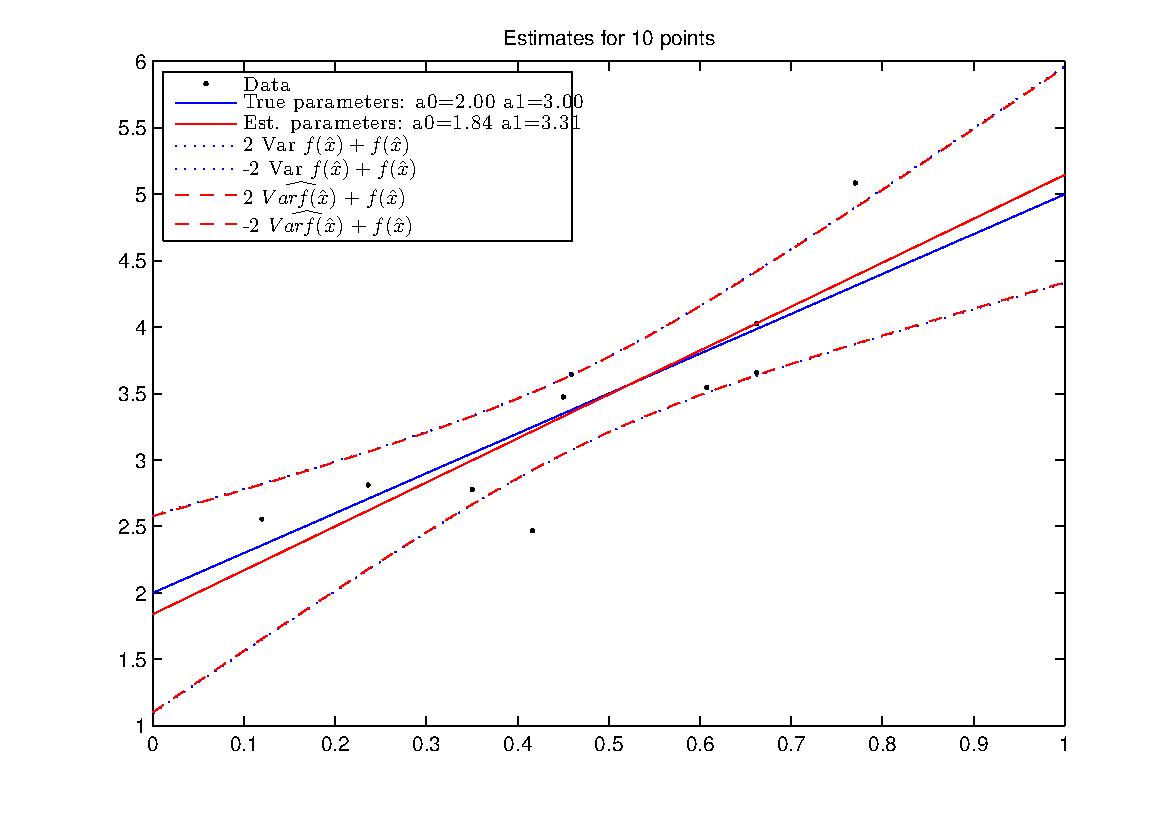
\includegraphics[width=.3\textwidth]{ten_point.pdf}
    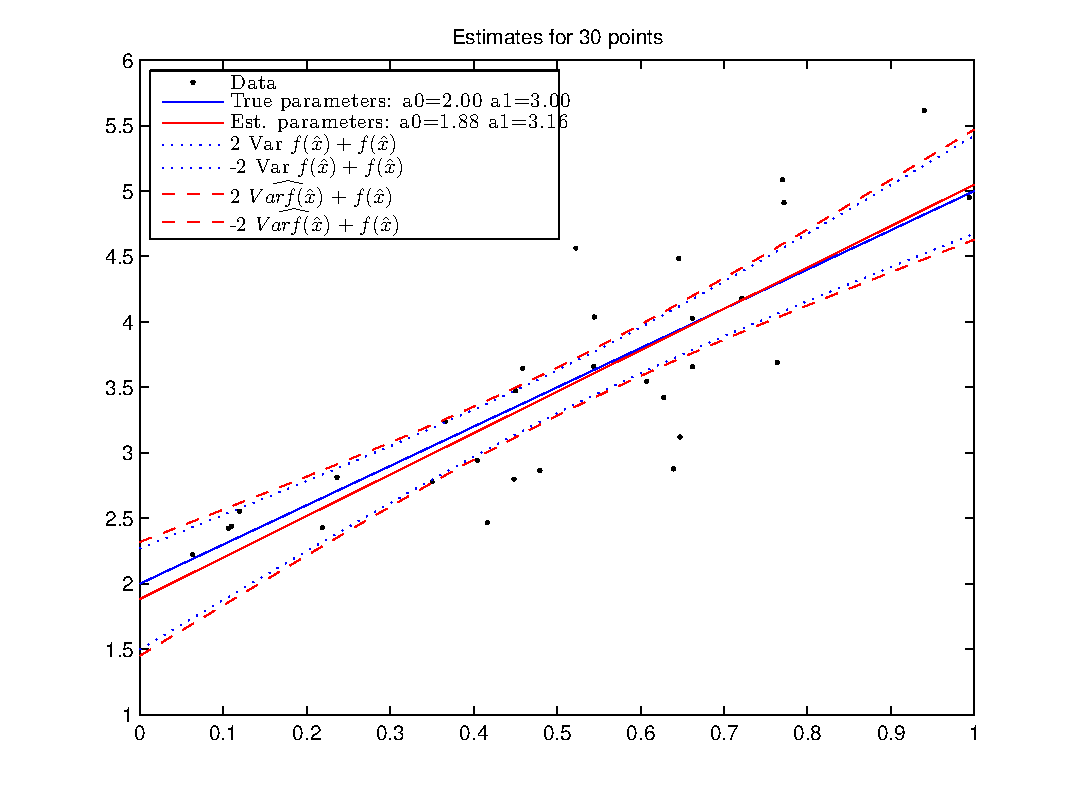
\includegraphics[width=.3\textwidth]{thirty_points.pdf}
    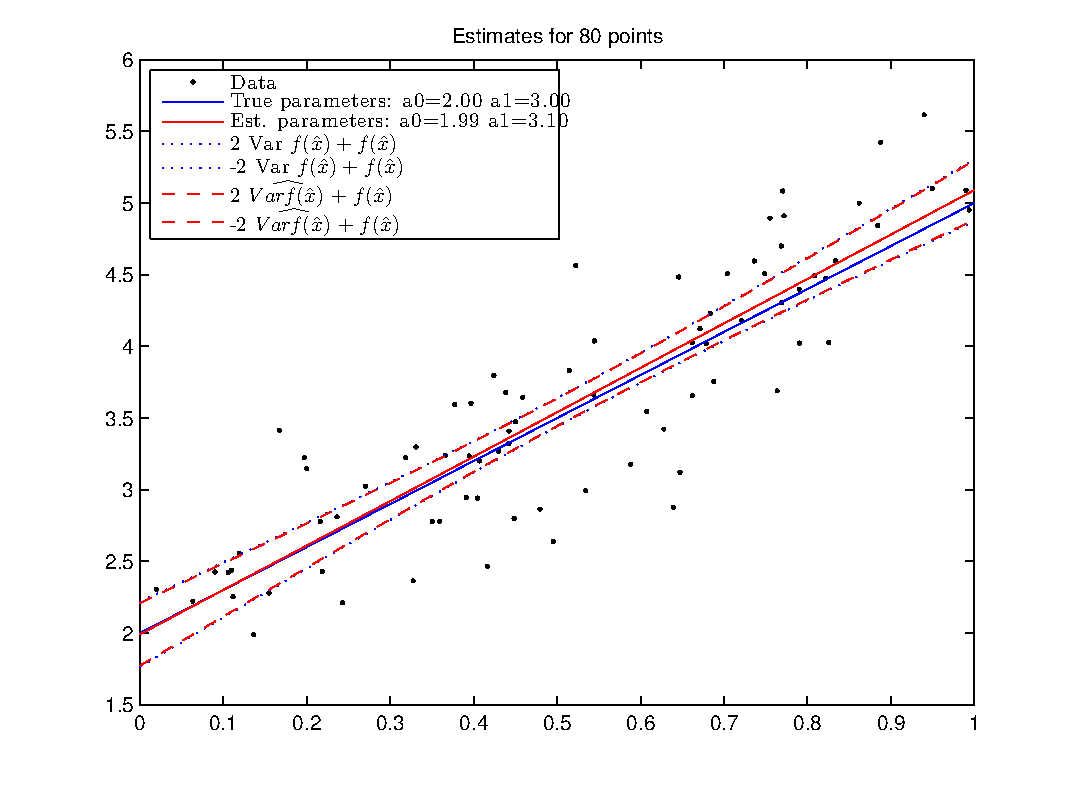
\includegraphics[width=.3\textwidth]{eighty_points.pdf}
    \captionof{figure}{Estimates and quantified uncertainty in them are illustrated for $n=10,30,80$ points. The data points $ax_i + b$ are shown as black points, the line $ax + b$ is shown in blue, and the estimated line $\hat a x + \hat b$ is shown in red.  The variance for each estimate $x$ when $\sigma^2$ is known is shown as a band with dotted blue lines with width $4\Var(\hat{f(x)})$. Similarly, the band for when $\sigma^2$ is unknown is shown with red dashed lines. Note that estimation for a given $x$ is most precise near $\mathrm E x_i = .5$}
\end{solution}

\definecolor{mygreen}{RGB}{28,172,0} % color values Red, Green, Blue
\definecolor{mylilas}{RGB}{170,55,241}
\lstset{language=Matlab,%
    %basicstyle=\color{red},
    breaklines=true,%
    morekeywords={matlab2tikz},
    keywordstyle=\color{blue},%
    morekeywords=[2]{1}, keywordstyle=[2]{\color{black}},
    identifierstyle=\color{black},%
    stringstyle=\color{mylilas},
    commentstyle=\color{mygreen},%
    showstringspaces=false,%without this there will be a symbol in the places where there is a space
    numbers=left,%
    numberstyle={\tiny \color{black}},% size of the numbers
    numbersep=9pt, % this defines how far the numbers are from the text
    emph=[1]{for,end,break},emphstyle=[1]\color{red}, %some words to emphasise
    %emph=[2]{word1,word2}, emphstyle=[2]{style},    
}
{
\footnotesize
\lstinputlisting[language=Matlab]{problem2.m}

\lstinputlisting[language=Matlab]{plot_estimates.m}
}
\end{document} 


